\documentclass{ltxdockit}[2011/03/25]
\usepackage{btxdockit}

\newcommand*{\biber}{\sty{biber}\xspace}
\newcommand*{\biblatex}{\sty{biblatex}\xspace}
\newcommand*{\biblatexml}{\sty{biblatexml}\xspace}
\newcommand*{\ris}{\sty{RIS}\xspace}
\newcommand*{\biblatexhome}{http://sourceforge.net/projects/biblatex/}
\newcommand*{\biblatexctan}{%
  http://www.ctan.org/tex-archive/macros/latex/contrib/biblatex/}
\usepackage{xr-hyper}
\externaldocument{biblatex}

\usepackage{fontspec}
\setmonofont{Courier New}
\setmainfont[Ligatures=TeX]{Linux Libertine O}
\setsansfont[Ligatures=TeX]{Linux Biolinum O}
\usepackage[american]{babel}
\usepackage[strict]{csquotes}
\usepackage{tabularx}
\usepackage{longtable}
\usepackage{booktabs}
\usepackage{shortvrb}
\usepackage{microtype}
\usepackage{typearea}
\usepackage{mdframed}
\usepackage{graphicx}
\usepackage[flushmargin]{footmisc}
\areaset[current]{370pt}{700pt}
\lstset{
    basicstyle=\ttfamily,
    commentstyle=\color{red}\ttfamily,
    keepspaces=true,
    upquote=true,
    frame=single,
    breaklines=true,
    postbreak=\raisebox{0ex}[0ex][0ex]{\ensuremath{\color{red}\hookrightarrow\space}}
}
\KOMAoptions{numbers=noenddot}
\addtokomafont{title}{\sffamily}
\addtokomafont{paragraph}{\spotcolor}
\addtokomafont{section}{\spotcolor}
\addtokomafont{subsection}{\spotcolor}
\addtokomafont{subsubsection}{\spotcolor}
\addtokomafont{descriptionlabel}{\spotcolor}
\setkomafont{caption}{\bfseries\sffamily\spotcolor}
\setkomafont{captionlabel}{\bfseries\sffamily\spotcolor}
\pretocmd{\cmd}{\sloppy}{}{}
\pretocmd{\bibfield}{\sloppy}{}{}
\pretocmd{\bibtype}{\sloppy}{}{}
\makeatletter
\patchcmd{\paragraph}
  {3.25ex \@plus1ex \@minus.2ex}{-3.25ex\@plus -1ex \@minus -.2ex}{}{}
\patchcmd{\paragraph}{-1em}{1.5ex \@plus .2ex}{}{}
\makeatother

\MakeAutoQuote{«}{»}
\MakeAutoQuote*{<}{>}
\MakeShortVerb{\|}

\newcommand*{\msecref}[1]{B:\secref{#1}}

\titlepage{%
  title={\biblatex Quickstart Guide},
  subtitle={},
  url={\biblatexhome},
  author={Philip Kime},
  email={},
  revision={1.0},
  date={\today}}

\hypersetup{%
  pdftitle={\biblatex Quickstart Guide},
  pdfsubject={Programmable Bibliographies and Citations},
  pdfauthor={Philip Kime},
  pdfkeywords={tex, latex, bibtex, bibliography, references, citation}}

% tables

\newcolumntype{H}{>{\sffamily\bfseries\spotcolor}l}
\newcolumntype{L}{>{\raggedright\let\\=\tabularnewline}p}
\newcolumntype{R}{>{\raggedleft\let\\=\tabularnewline}p}
\newcolumntype{C}{>{\centering\let\\=\tabularnewline}p}
\newcolumntype{V}{>{\raggedright\let\\=\tabularnewline\ttfamily}p}

\newcommand*{\sorttablesetup}{%
  \tablesetup
  \ttfamily
  \def\new{\makebox[1.25em][r]{\ensuremath\rightarrow}\,}%
  \def\alt{\par\makebox[1.25em][r]{\ensuremath\hookrightarrow}\,}%
  \def\note##1{\textrm{##1}}}

\newcommand{\tickmarkyes}{\Pisymbol{psy}{183}}
\newcommand{\tickmarkno}{\textendash}
\providecommand*{\textln}[1]{#1}
\providecommand*{\lnstyle}{}

% markup and misc

\setcounter{secnumdepth}{4}

% following snippet is based on code by Michael Ummels (TeX Stack Exchange)
% <http://tex.stackexchange.com/a/13073/8305>
\makeatletter
  \newcommand\fnurl@[1]{\footnote{\url@{#1}}}
  \DeclareRobustCommand{\fnurl}{\hyper@normalise\fnurl@}
\makeatother

\begin{document}

\printtitlepage
\tableofcontents
\listoftables

\newpage
\section{Introduction}
\label{int}
\biblatex is a bibliography system for \latex users. It surpasses the facilities provided by \bibtex and provides a very large feature set which can be somewhat overwhelming to the new user. This quick start guide aims to demonstrate the basic setup of \biblatex along with a selection of «how to» guides for common things which users typically need to do.

\biblatex tracks the citations you make in your document and the options you set to control how the citations are managed. It passes these to a backend processor \biber\footnote{At time of writing, \biblatex supports two backend processors, \biber and legacy \bibtex. New users, who are the focus audience for this guide, should use \biber.} which performs some tasks and then writes out a sorted representation of the bibliography data. \biblatex then uses this information on subsequent runs of \latex to format and print a bibliography. You can see the general workflow in figure \ref{fig1}.

See the appendix \secref{apx:hist} for some history about how \biblatex started, and how it differs from \bibtex. References to the main \biblatex documentation file are formatted as follows below: \msecref{int}.

\section{Getting Started}

Using \biblatex is easy. Here is a basic example:

\begin{ltxexample}[style=latex]{}
\documentclass{article}

% Load the package
\usepackage{biblatex}

% Tell biblatex the name of your
% bibliography database file
\addbibresource{refs.bib}
\begin{document}

% Mention some bibliography items
% in your text ...
Someone said something interesting
in \cite{work1} and also in \cite{work2}.

% Print the bibliography
\printbibliography
\end{document}
\end{ltxexample}
%
You would run the \latex engine of your choice\footnote{Typically one of \texttt{pdflatex}, \texttt{xelatex} or \texttt{lualatex}} on this file, then run \biber on the \file{.bcf} file this produces and then your \latex engine once more\footnote{Often two or more times in fact, depending on the \biblatex options chosen which may require more runs to resolve various references.}. The commands you run would look like this assuming the file above was called \file{test.tex}.

\begin{verbatim}
latex test
biber test
latex text
latex text
\end{verbatim}
%
Notice that we didn't need to specify the file extensions as \latex knows to look for the \file{.tex} file and \biber knows to look for the \file{.bcf} file. So, this is all equivalent to doing:

\begin{verbatim}
latex test.tex
biber test.bcf
latex text.tex
latex text.tex
\end{verbatim}
%
Many people will be using \latex editing applications which hide these commands from you anyway and which will be activated by keyboard shortcuts or menu items.

One thing that \biblatex is good at is \emph{localisation}, that is, knowing what to do when switching between languages. If you are using any language other than basic English, then you should be loading \sty{inputenc} (\texttt{pdflatex}) or \sty{fontspec} (\texttt{xelatex} or \texttt{lualatex}) and then one or other of the \sty{babel} or \sty{polyglossia} packages for multi-language support. \biblatex knows how to connect with \sty{babel} and \sty{polyglossia} and can use their facilities for switching language handling and even font scripts dynamically in the bibliography and in citations. For example if you were writing in French, using \texttt{lualatex} as the engine and \sty{polyglossia} as your language support package, your basic document would look like this:

\begin{ltxexample}[style=latex]{}
\documentclass{article}
\usepackage{polyglossia}
\setdefaultlanguage{french}
\usepackage{fontspec}
\usepackage{biblatex}
\addbibresource{refs.bib}

\begin{document}

Someone said something interesting
in \cite{work1} and also in \cite{work2}.

\printbibliography
\end{document}
\end{ltxexample}
%
Language packages like \sty{babel} and \sty{polyglossia} should be loaded \emph{before} \biblatex so that it can detect which one you are using.

It is also recommended to use the \sty{csquotes} package as this integrates with \biblatex to provide sophisticated combined citation/quotation macros are also multi-lingual aware. So, if you were to settle on a document skeleton for biblatex use with \texttt{xelatex} or \texttt{lualatex}, it might look like this:

\begin{ltxexample}[style=latex]{}
\documentclass{article}
\usepackage{polyglossia}
\setdefaultlanguage{english}
\usepackage{fontspec}
\usepackage{biblatex}
\usepackage{csquotes}
\addbibresource{refs.bib}

\begin{document}

Someone said something interesting
in \cite{work1} and also in \cite{work2}.

\printbibliography
\end{document}
\end{ltxexample}
%
Or with \texttt{pdflatex}, like this:

\begin{ltxexample}[style=latex]{}
\documentclass{article}
\usepackage{polyglossia}
\setdefaultlanguage{english}
\usepackage[T1]{fontenc}
\usepackage[utf8]{inputenc}
\usepackage{biblatex}
\addbibresource{refs.bib}

\begin{document}

Someone said something interesting
in \cite{work1} and also in \cite{work2}.

\printbibliography
\end{document}
\end{ltxexample}
%
See the main \biblatex manual \ref{int:pre} for details about required, recommended or incompatible packages. \biblatex comes with many example files which are placed in the \path{doc/latex/biblatex/examples} subdirectory of the \file{texmf} tree. These are annotated and very useful for learning how to do various things.

\section{Changing Things \ldots}

The \biblatex package options are detailed in the \biblatex manual (\msecref{use}).

\subsection{Choosing a style}

The first option you will want to specify is the \opt{style} option. This decides the formatting of your bibliography and citations. There are several standard styles which \biblatex offers (\msecref{use:xbx}). 

\begin{ltxexample}[style=latex]{}
\usepackage[style=authoryear]{biblatex}
\end{ltxexample}
%
You may have separate styles for the bibliograpy and citations by using the \opt{bibstyle} and \opt{citestyle} options respectively. \opt{style} sets both \opt{bibstyle} and \opt{citestyle}:

\begin{ltxexample}[style=latex]{}
\usepackage[citestyle=authoryear, bibstyle=authortitle]{biblatex}
\end{ltxexample}

\subsection{Migrating from natbib}
\biblatex has a compatibility setting which you can use to emulate standard \sty{natbib} commands (\msecref{use:cit:nat}) and it is enabled like this:

\begin{ltxexample}[style=latex]{}
\usepackage[natbib=true]{biblatex}
\end{ltxexample}

\subsection{Sorting the bibliography}

One of the main purposes of a bibliography system is to sort the bibliography correctly. This might be by author names in a humanties paper or by a label or number for a physical sciences paper, for example. Sorting with \biblatex is completely customisable and very sophisticated, supporting full Unicode\footnote{Using an implementation of the Unicode Collation Algorithm (UCA) with Common Locale Data Repository (CLDR) tailoring.} Sorting is done by defining a sorting «scheme», which is given a name. The scheme name is then used as the value of the sorting options. To set the default, global sorting scheme, use the \opt{sorting} package option:

\begin{ltxexample}[style=latex]{}
\usepackage[sorting=ynt]{biblatex}
\end{ltxexample}
%
There are several pre-defined sorting schemes (\msecref{use:opt:pre:gen}). You may also define your own sorting schemes (\msecref{aut:ctm:srt}) or override the global sorting scheme and use different sorting schemes for different bibliography lists (\msecref{use:bib:context}).

% \begin{lstlisting}[style=bibtex]{}
% \end{lstlisting}


\appendix
\section*{Appendix}
\addcontentsline{toc}{section}{Appendix}

\section{History}
\label{apx:hist}
\biblatex was developed to allow bibliography styles to be created using
\TeX macros rather than the somewhat obscure and tricky stack language used
in \bibtex \file{.bst} style files. It is very important to distinguish
between \bibtex the \emph{program} and \bibtex the \emph{file format}.
«\bibtex» is the name of a program which generates a bibliography file (\file{.bbl}) for you document. \bibtex the program does five main things:

\begin{enumerate}
\item Reads the \file{.aux} to find out what citations were used
\item Reads the \file{.bib} bibliography data file to retrieve bibliography entry data
\item Sorts the bibliography entries
\item Applies some formatting style (\file{.bst}) to the entries
\item Writes the results to the \file{.bbl} file
\end{enumerate}
%
\biblatex takes over task 4 and replaces it with a sophisticated set of \latex macros which define bibliography styles. This makes styles much easier to write and to customise. Initially, \biblatex still used \bibtex (the program) to perform tasks 1,2,3 and 5 with the difference that the resulting \file{.bbl} does not contain a printable bibliography but rather something like a sorted database, using \TeX macros, to which the \biblatex styles are applied. \biblatex does this by using only one special \bibtex \file{.bst} «style» file which describes this file format. 

In a sense, \biblatex abused \bibtex for its data reading and sorting functions while ignoring arguably its main function of formatting bibliographic data. In 2008, development on \biber started which aimed to provide a dedicated and customised backend for \biblatex to remove the dependency on \bibtex. The goals were:

\begin{itemize}
\item Full Unicode support, which is lacking in all \bibtex (the program) variants to some degree
\item Better, more flexible sorting algorithm
\item Customisable interface file format to allow far more options than are possible with \bibtex (the progam)
\end{itemize}
%
\biber now fulfills these goals along with a large additional feature set. \biblatex with \biber still supports (and always will) the \bibtex file format (\file{.bib}) as this is the most widely used format in the \latex world. However, it is not limited to this and supports other data formats with a modular internal design to allow relatively easy addition of other data formats.

\biber takes over all of the tasks previously done by \bibtex for \biblatex. One change is that \biber does not read the \file{.aux} file but reads a more complex and structured file which \biblatex uses to pass information to \biber. This is the XML format \file{.bcf}, the Biblatex Control File. See Figure \ref{fig1} for an overview.

\begin{figure}
  \centering
  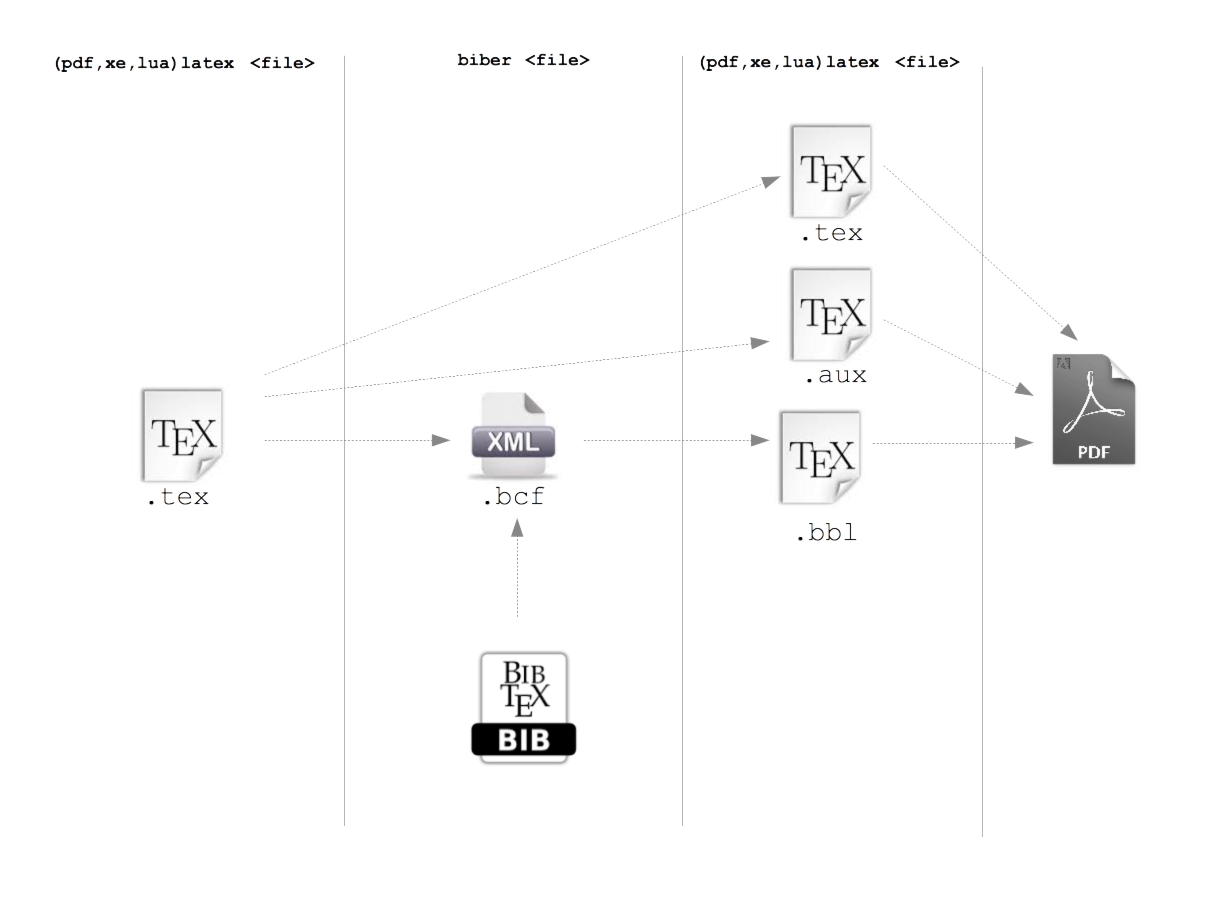
\includegraphics[width=\textwidth,keepaspectratio=true]{qs1.png}
  \caption{biblatex workflow}
  \label{fig1}
\end{figure}

\end{document}
%%% Local Variables:
%%% coding: utf-8
%%% eval: (auto-fill-mode -1)
%%% eval: (visual-line-mode)
%%% End:
